\subsection{Learning interpretable representations}
\label{hsicindep}
Suppose we want to summarize the data $x$ with two independent components $u$ and $v$, as shown in Figure~\ref{hsicpgm}a. The task is especially important for data exploration since independent representations are often more easily interpreted.

A related problem is finding latent factors $(z^1, ..., z^d)$ that correspond to real and interpretable variations in the data. Learning independent representations is then a key step towards learning \emph{disentangled} representations~\cite{betatcVAE, Higgins2017, Kim2018, Chen2016}.
The $\beta$-VAE~\cite{Higgins2017} proposes further penalizing the $\kld{q_\phi(z\mid x)}{p(z)}$ term. It attains significant improvement over state-of-the art methods on real datasets. However, this penalization has been shown to yield poor reconstruction performance~\cite{Burgess2018}. The $\beta$-TCVAE~\cite{betatcVAE} penalized an approximation of the \textit{total correlation} (TC), defined as  $\kld{\hat{q}_\phi(z)}{\prod_k \hat{q}_\phi(z^k)}$ ~\cite{Watanabe}, which is a measure of multivariate mutual independence. However, this quantity does not have a closed-form solution~\cite{Durrieu2012} and the $\beta$-TCVAE uses a biased estimator of the TC---a lower bound from Jensen inequality. That bias will be zero only if evaluated on the whole dataset, which is not possible since the estimator has quadratic complexity in the number of samples. However, the bias from the HSIC~\cite{HSIC} is of order $\mathcal{O}(\nicefrac{1}{n})$; it is negligible whenever the batch-size is large enough. HSIC therefore appears to be a more suitable method to enforce independence in the latent space.

To assess the performance of these various approaches to finding independent representations, we consider a linear Gaussian system, for which exact posterior inference is tractable. Let $(n, m, d) \in \mathbb{N}^3$ and $\lambda \in \mathbb{R}^+$. Let $(A, B) \in \mathbb{R}^{d\times n}\times\mathbb{R}^{d\times m}$ be random matrices with iid normal entries. Let $\Sigma \in \mathbb{R}^{d\times d}$ be a random matrix following a Wishart distribution. Consider the following generative model:
\begin{equation}
\begin{split}
v &\sim \textrm{Normal}(0, I_n) \\
u &\sim \textrm{Normal}(0, I_m) \\
x\mid u, v &\sim \textrm{Normal}(Av + Bu, \lambda I_d + \Sigma).
\end{split}
\end{equation}

The marginal log-likelihood $p(x)$ is tractable:
\begin{equation}
x \sim \textrm{Normal}(0, \lambda I_d + \Sigma + AA^T + BB^T). 
\end{equation}

The complete posterior $p(u, v \mid x)$ is tractable via block matrix inversion, as is the marginal $p(x)$:
\begin{equation}
\begin{split}
V^{-1} &= I_{n+m} + [A, B]^T (\lambda I_d + \Sigma)^{-1} [A, B]  \\
H_\mu &= \Sigma [A, B]^T (\lambda I_d + \Sigma)^{-1} \\
u, v \mid x &\sim \textrm{Normal}(H_\mu x, V). 
\end{split}
\end{equation}

We apply HCV with:
\begin{align}
    Z = \{u, v\}, X = \{x\}, S = \emptyset , \mathcal{Z}_0 = \{u, v\}\text{, and } \mathcal{S}_0 = \emptyset.
\end{align}
This is equivalent to adding to the ELBO the penalty:
\begin{align}
- \lambda \text{HSIC}(\mathbb{E}_{p_\text{data}(x)}q_\phi(u, v\mid x))
\end{align}. We report the trade-off between correlation of the representation and the ELBO for various penalty weights $\lambda$ for each algorithm: $\beta$-VAE~\cite{Higgins2017}, $\beta$-TCVAE~\cite{betatcVAE}, an unconstrained VAE, and HCV. As correlation measures, we consider the summed Pearson correlation $\sum_{(i, j)}\rho(\hat{q}_\phi(u^i), \hat{q}_\phi(v^j))$ and HSIC.

\begin{figure}[ht]
\captionsetup[subfigure]{justification=centering}
    \centering  
    \begin{subfigure}[t]{0.5\textwidth}
        \centering   
		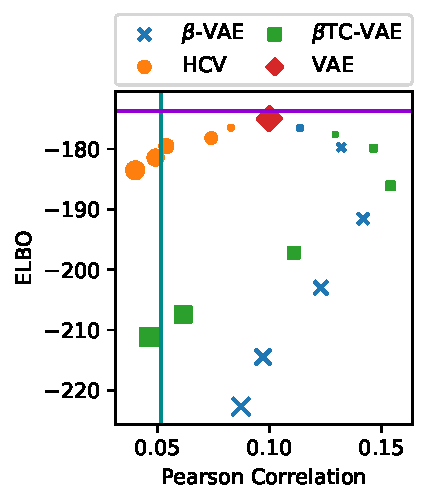
\includegraphics[width=0.7\textwidth]{figures/gaussian.pdf}
    \end{subfigure}%
    ~  
    \begin{subfigure}[t]{0.5\textwidth}
        \centering  
		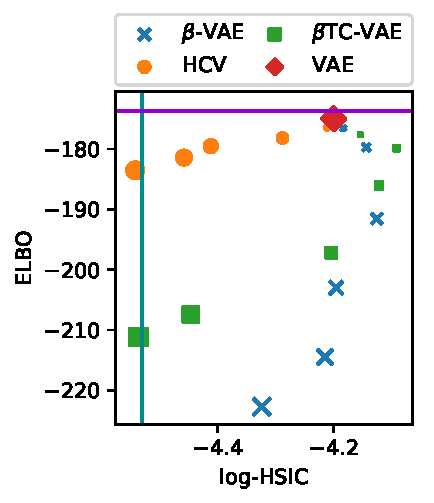
\includegraphics[width=0.7\textwidth]{figures/gaussian_hsic.pdf}
    \end{subfigure}

    \caption[Results for the linear Gaussian system]{Results for the linear Gaussian system. All results are for a test set. Each dot is averaged across five random seeds. Larger dots indicate greater regularization. The purple line is the log-likelihood under the true posterior. The cyan line is the correlation under the true posterior.}
    %\vspace{-0.5cm}
    \label{hsiclingaussfigure}
\end{figure}

Results are reported in Figure~\ref{hsiclingaussfigure}. The VAE baseline (like all the other methods) has an ELBO value worse than the marginal log-likelihood (horizontal bar) since the real posterior is not likely to be in the function class given by naive mean field AEVB. Also, this baseline has a greater dependence in the aggregated posterior $\hat{q}_\phi(u, v)$ than in the exact posterior $\hat{p}(u, v)$ (vertical bar) for the two measures of correlation. Second, while correcting the variational posterior, we want the best trade-off between model fit and independence. HCV attains the highest ELBO values despite having the lowest correlation. 






